\subsection{Scenario 1: No Changes}
\textit{In this scenario, no external changes are made to the infrastructure. The purpose of this scenario is to see how the system behaves when no changes are made.}

To introduce the graphs and what they mean, this subsection will go through the graphs in a bit more detail than in the subsections afterwards. 

\begin{figure}[H]
    \centering
    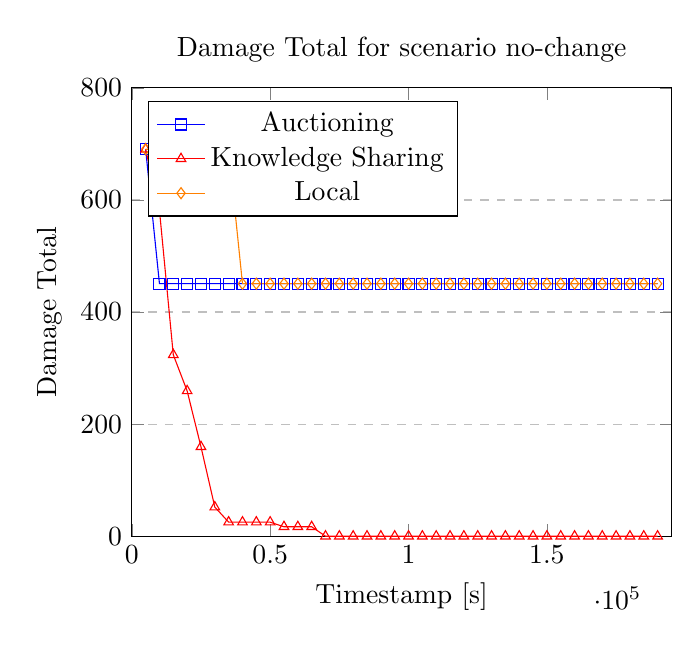
\begin{tikzpicture}
\begin{axis}[
    title={Damage Total for scenario no-change},
    xlabel={Timestamp [s]},
    ylabel={Damage Total},
    xmin=0, xmax=195000,
    ymin=0, ymax=800,
    legend pos=north west,
    ymajorgrids=true,
    grid style=dashed,
]

\addplot[
    color=blue,
    mark=square,
    ]
    coordinates {
    (5000,690.52)(10000,450.57)(15000,450.57)(20000,450.57)(25000,450.57)(30000,450.57)(35000,450.57)(40000,450.57)(45000,450.57)(50000,450.57)(55000,450.57)(60000,450.57)(65000,450.57)(70000,450.57)(75000,450.57)(80000,450.57)(85000,450.57)(90000,450.57)(95000,450.57)(100000,450.57)(105000,450.57)(110000,450.57)(115000,450.57)(120000,450.57)(125000,450.57)(130000,450.57)(135000,450.57)(140000,450.57)(145000,450.57)(150000,450.57)(155000,450.57)(160000,450.57)(165000,450.57)(170000,450.57)(175000,450.57)(180000,450.57)(185000,450.57)(190000,450.57)
    };
    \addlegendentry{Auctioning}
\addplot[
    color=red,
    mark=triangle,
    ]
    coordinates {
    (5000,690.52)(10000,581.45)(15000,323.71)(20000,259.27)(25000,159.58)(30000,51.98)(35000,25.08)(40000,25.08)(45000,25.08)(50000,25.08)(55000,16.82)(60000,16.82)(65000,16.82)(70000,0.00)(75000,0.00)(80000,0.00)(85000,0.00)(90000,0.00)(95000,0.00)(100000,0.00)(105000,0.00)(110000,0.00)(115000,0.00)(120000,0.00)(125000,0.00)(130000,0.00)(135000,0.00)(140000,0.00)(145000,0.00)(150000,0.00)(155000,0.00)(160000,0.00)(165000,0.00)(170000,0.00)(175000,0.00)(180000,0.00)(185000,0.00)(190000,0.00)
    };
    \addlegendentry{Knowledge Sharing}
\addplot[
    color=orange,
    mark=diamond,
    ]
    coordinates {
    (5000,690.52)(10000,690.52)(15000,690.52)(20000,690.52)(25000,690.52)(30000,690.52)(35000,690.52)(40000,450.57)(45000,450.57)(50000,450.57)(55000,450.57)(60000,450.57)(65000,450.57)(70000,450.57)(75000,450.57)(80000,450.57)(85000,450.57)(90000,450.57)(95000,450.57)(100000,450.57)(105000,450.57)(110000,450.57)(115000,450.57)(120000,450.57)(125000,450.57)(130000,450.57)(135000,450.57)(140000,450.57)(145000,450.57)(150000,450.57)(155000,450.57)(160000,450.57)(165000,450.57)(170000,450.57)(175000,450.57)(180000,450.57)(185000,450.57)(190000,450.57)
    };
    \addlegendentry{Local}
    
\end{axis}
\end{tikzpicture}
    \caption{This graph shows the overall damage of the system in the scenario where no changes are made overtime.}
    \label{fig:overall-damage-no-change}
\end{figure}

From figure \ref{fig:overall-damage-no-change} we see that the agent with the Local-feature set (from here-on \textit{local-agent}) slowly reduces the overall damage of the network, but is unable to get any lower than around $4.000$, and stays at this value after roughly the first $150$ seconds.
After roughly the first $100$ seconds, both the auctioning and knowledge-sharing agents are able to almost reach zero. The lowest value is for the knowledge-sharing agent at  $5\%$ ($215$ damage total) of the damage the local-agent.

\begin{figure}[H]
    \centering
    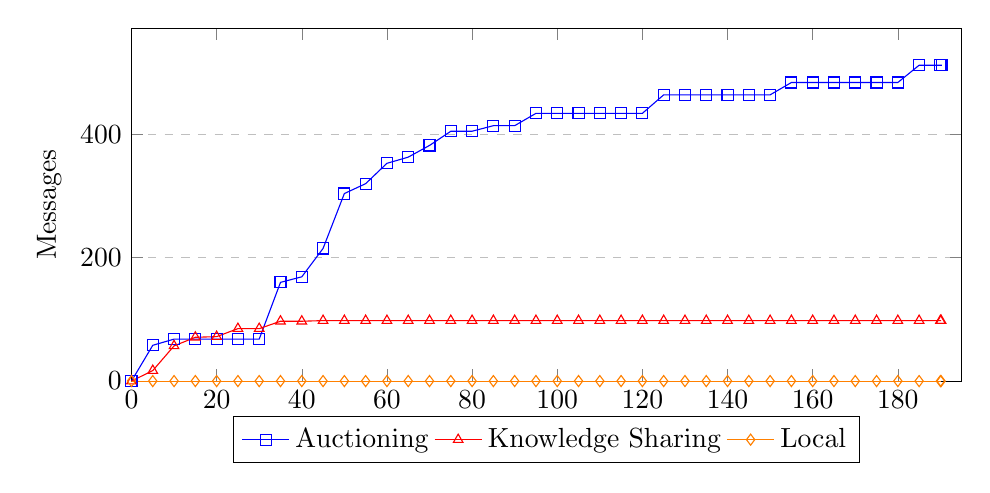
\begin{tikzpicture}
\begin{axis}[
    xlabel={Timestamp [s]},
    ylabel={Messages},
    xmin=0, xmax=195000,
    ymin=0, ymax=572,
    legend columns=-1,
    legend style={at={(0.5,-0.1)},anchor=north},
    ymajorgrids=true,
    grid style=dashed,
    width=\textwidth,
    height=0.5\textwidth,
    scaled x ticks=base 10:-3,
    xtick scale label code/.code={}
]

	\addplot[color=blue,mark=square] coordinates {
        (0,0)(5000,58)(10000,68)(15000,68)(20000,68)(25000,68)(30000,68)(35000,160)(40000,169)(45000,215)(50000,304)(55000,320)(60000,353)(65000,363)(70000,382)(75000,405)(80000,405)(85000,414)(90000,414)(95000,434)(100000,434)(105000,434)(110000,434)(115000,434)(120000,434)(125000,464)(130000,464)(135000,464)(140000,464)(145000,464)(150000,464)(155000,484)(160000,484)(165000,484)(170000,484)(175000,484)(180000,484)(185000,512)(190000,512)(190364,512)
    };
    \addlegendentry{Auctioning}
	\addplot[color=red,mark=triangle] coordinates {
        (0,0)(5000,17)(10000,57)(15000,71)(20000,72)(25000,85)(30000,85)(35000,97)(40000,97)(45000,98)(50000,98)(55000,98)(60000,98)(65000,98)(70000,98)(75000,98)(80000,98)(85000,98)(90000,98)(95000,98)(100000,98)(105000,98)(110000,98)(115000,98)(120000,98)(125000,98)(130000,98)(135000,98)(140000,98)(145000,98)(150000,98)(155000,98)(160000,98)(165000,98)(170000,98)(175000,98)(180000,98)(185000,98)(190000,98)(190165,98)
    };
    \addlegendentry{Knowledge Sharing}
	\addplot[color=orange,mark=diamond] coordinates {
        (0,0)(5000,0)(10000,0)(15000,0)(20000,0)(25000,0)(30000,0)(35000,0)(40000,0)(45000,0)(50000,0)(55000,0)(60000,0)(65000,0)(70000,0)(75000,0)(80000,0)(85000,0)(90000,0)(95000,0)(100000,0)(105000,0)(110000,0)(115000,0)(120000,0)(125000,0)(130000,0)(135000,0)(140000,0)(145000,0)(150000,0)(155000,0)(160000,0)(165000,0)(170000,0)(175000,0)(180000,0)(185000,0)(190000,0)(190150,0)
    };
    \addlegendentry{Local}




\end{axis}
\end{tikzpicture}
    \caption{Graph showing the total amount of messages sent between agents in the scenario where no changes are made overtime.}
    \label{fig:messages-no-change}
\end{figure}

In figure \ref{fig:messages-no-change} we can see that the local-agent shares no messages, as this feature-set does not allow for it. The auctioning agent sends the most messages, almost three times as much as the knowledge-sharing agents. This can be explained by the fact that the auctioning agents have a total of $11$ events that can be sent to other agents, compared to the knowledge-sharing agent, which has only $4$ types of messages. This $4 / 11$ ratio is roughly the same as the ratio between the amount of messages sent by the auctioning and knowledge-sharing agents. However, this could be a coincidence, and more research would be needed for this assumption. During an auction participating nodes send on average $4$ messages per participating node, which could also explain the difference in messages sent. 

\begin{figure}[H]
    \centering
    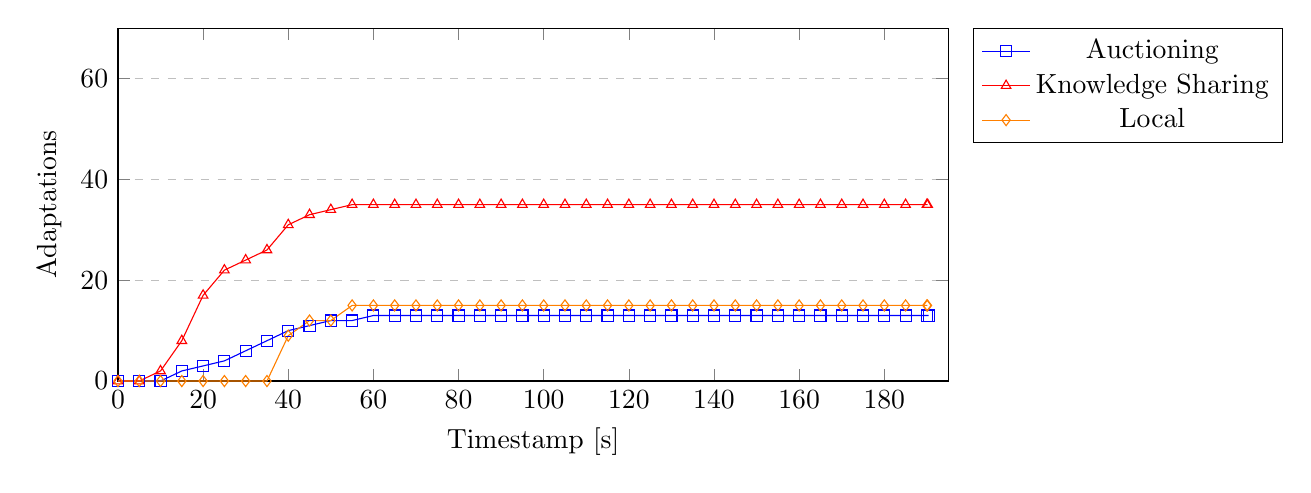
\begin{tikzpicture}
\begin{axis}[
    xlabel={Timestamp [s]},
    ylabel={Adaptations},
    xmin=0, xmax=195000,
    ymin=0, ymax=70,
    legend pos=outer north east,
    ymajorgrids=true,
    grid style=dashed,
    width=\textwidth,
    height=0.5\textwidth,
    scaled x ticks=base 10:-3,
    xtick scale label code/.code={}
]

	\addplot[color=blue,mark=square] coordinates {
        (0,0)(5000,0)(10000,0)(15000,2)(20000,3)(25000,4)(30000,6)(35000,8)(40000,10)(45000,11)(50000,12)(55000,12)(60000,13)(65000,13)(70000,13)(75000,13)(80000,13)(85000,13)(90000,13)(95000,13)(100000,13)(105000,13)(110000,13)(115000,13)(120000,13)(125000,13)(130000,13)(135000,13)(140000,13)(145000,13)(150000,13)(155000,13)(160000,13)(165000,13)(170000,13)(175000,13)(180000,13)(185000,13)(190000,13)(190434,13)
    };
    \addlegendentry{Auctioning}
	\addplot[color=red,mark=triangle] coordinates {
        (0,0)(5000,0)(10000,2)(15000,8)(20000,17)(25000,22)(30000,24)(35000,26)(40000,31)(45000,33)(50000,34)(55000,35)(60000,35)(65000,35)(70000,35)(75000,35)(80000,35)(85000,35)(90000,35)(95000,35)(100000,35)(105000,35)(110000,35)(115000,35)(120000,35)(125000,35)(130000,35)(135000,35)(140000,35)(145000,35)(150000,35)(155000,35)(160000,35)(165000,35)(170000,35)(175000,35)(180000,35)(185000,35)(190000,35)(190190,35)
    };
    \addlegendentry{Knowledge Sharing}
	\addplot[color=orange,mark=diamond] coordinates {
        (0,0)(5000,0)(10000,0)(15000,0)(20000,0)(25000,0)(30000,0)(35000,0)(40000,9)(45000,12)(50000,12)(55000,15)(60000,15)(65000,15)(70000,15)(75000,15)(80000,15)(85000,15)(90000,15)(95000,15)(100000,15)(105000,15)(110000,15)(115000,15)(120000,15)(125000,15)(130000,15)(135000,15)(140000,15)(145000,15)(150000,15)(155000,15)(160000,15)(165000,15)(170000,15)(175000,15)(180000,15)(185000,15)(190000,15)(190138,15)
    };
    \addlegendentry{Local}




\end{axis}
\end{tikzpicture}
    \caption{Graph showing the total amount of adaptations applied by agents in the scenario where no changes are made overtime.}
    \label{fig:proposals-no-change}
\end{figure}

From figure \ref{fig:proposals-no-change} we can see that auctioning and knowledge-sharing agent both roughly have the same amount of adaptations applied. The local-agent is only able to apply a handful of adaptations.

\begin{figure}[H]
    \centering
        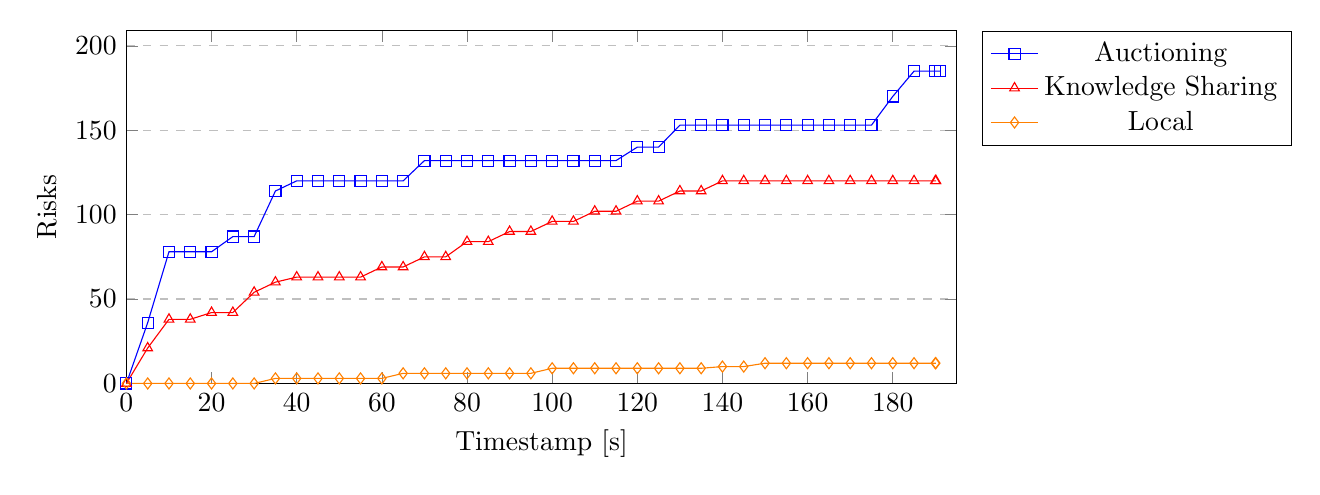
\begin{tikzpicture}
\begin{axis}[
    xlabel={Timestamp [s]},
    ylabel={Risks},
    xmin=0, xmax=195000,
    ymin=0, ymax=209,
    legend pos=outer north east,
    ymajorgrids=true,
    grid style=dashed,
    width=\textwidth,
    height=0.5\textwidth,
    scaled x ticks=base 10:-3,
    xtick scale label code/.code={}
]

	\addplot[color=blue,mark=square] coordinates {
        (0,0)(5000,36)(10000,78)(15000,78)(20000,78)(25000,87)(30000,87)(35000,114)(40000,120)(45000,120)(50000,120)(55000,120)(60000,120)(65000,120)(70000,132)(75000,132)(80000,132)(85000,132)(90000,132)(95000,132)(100000,132)(105000,132)(110000,132)(115000,132)(120000,140)(125000,140)(130000,153)(135000,153)(140000,153)(145000,153)(150000,153)(155000,153)(160000,153)(165000,153)(170000,153)(175000,153)(180000,170)(185000,185)(190000,185)(191066,185)
    };
    \addlegendentry{Auctioning}
	\addplot[color=red,mark=triangle] coordinates {
        (0,0)(5000,21)(10000,38)(15000,38)(20000,42)(25000,42)(30000,54)(35000,60)(40000,63)(45000,63)(50000,63)(55000,63)(60000,69)(65000,69)(70000,75)(75000,75)(80000,84)(85000,84)(90000,90)(95000,90)(100000,96)(105000,96)(110000,102)(115000,102)(120000,108)(125000,108)(130000,114)(135000,114)(140000,120)(145000,120)(150000,120)(155000,120)(160000,120)(165000,120)(170000,120)(175000,120)(180000,120)(185000,120)(190000,120)(190155,120)
    };
    \addlegendentry{Knowledge Sharing}
	\addplot[color=orange,mark=diamond] coordinates {
        (0,0)(5000,0)(10000,0)(15000,0)(20000,0)(25000,0)(30000,0)(35000,3)(40000,3)(45000,3)(50000,3)(55000,3)(60000,3)(65000,6)(70000,6)(75000,6)(80000,6)(85000,6)(90000,6)(95000,6)(100000,9)(105000,9)(110000,9)(115000,9)(120000,9)(125000,9)(130000,9)(135000,9)(140000,10)(145000,10)(150000,12)(155000,12)(160000,12)(165000,12)(170000,12)(175000,12)(180000,12)(185000,12)(190000,12)(190110,12)
    };
    \addlegendentry{Local}




\end{axis}
\end{tikzpicture}
    \caption{Graph showing the number of unique risks detected by agents in the scenario where no changes are made overtime.}
    \label{fig:risk-count-no-change}
\end{figure}

Figure \ref{fig:risk-count-no-change} shows that the auctioning-agent detects the most risks, followed by the knowledge-sharing agent with only $30\%$ of the risks found. The local-agent detects the least amount of risks at only $10\%$ compared to the auctioning agent. It is to be expected that the local-agents can only detect a fraction of what the other agents detect, as the risks that can be deduced from only their local knowledge is limited.

\begin{figure}[H]
    \centering
        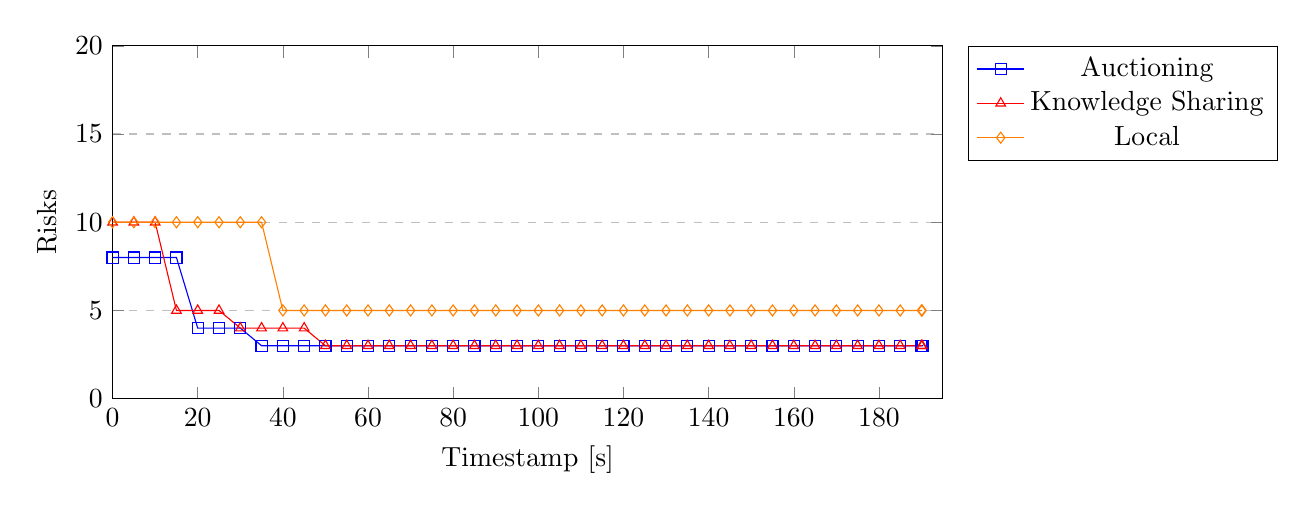
\begin{tikzpicture}
\begin{axis}[
    xlabel={Timestamp [s]},
    ylabel={Risks},
    xmin=0, xmax=195000,
    ymin=0, ymax=20,
    legend pos=outer north east,
    ymajorgrids=true,
    grid style=dashed,
    width=\textwidth,
    height=0.5\textwidth,
    scaled x ticks=base 10:-3,
    xtick scale label code/.code={}
]

	\addplot[color=blue,mark=square] coordinates {
        (0,8)(5000,8)(10000,8)(15000,8)(20000,4)(25000,4)(30000,4)(35000,3)(40000,3)(45000,3)(50000,3)(55000,3)(60000,3)(65000,3)(70000,3)(75000,3)(80000,3)(85000,3)(90000,3)(95000,3)(100000,3)(105000,3)(110000,3)(115000,3)(120000,3)(125000,3)(130000,3)(135000,3)(140000,3)(145000,3)(150000,3)(155000,3)(160000,3)(165000,3)(170000,3)(175000,3)(180000,3)(185000,3)(190000,3)(190439,3)
    };
    \addlegendentry{Auctioning}
	\addplot[color=red,mark=triangle] coordinates {
        (0,10)(5000,10)(10000,10)(15000,5)(20000,5)(25000,5)(30000,4)(35000,4)(40000,4)(45000,4)(50000,3)(55000,3)(60000,3)(65000,3)(70000,3)(75000,3)(80000,3)(85000,3)(90000,3)(95000,3)(100000,3)(105000,3)(110000,3)(115000,3)(120000,3)(125000,3)(130000,3)(135000,3)(140000,3)(145000,3)(150000,3)(155000,3)(160000,3)(165000,3)(170000,3)(175000,3)(180000,3)(185000,3)(190000,3)(190147,3)
    };
    \addlegendentry{Knowledge Sharing}
	\addplot[color=orange,mark=diamond] coordinates {
        (0,10)(5000,10)(10000,10)(15000,10)(20000,10)(25000,10)(30000,10)(35000,10)(40000,5)(45000,5)(50000,5)(55000,5)(60000,5)(65000,5)(70000,5)(75000,5)(80000,5)(85000,5)(90000,5)(95000,5)(100000,5)(105000,5)(110000,5)(115000,5)(120000,5)(125000,5)(130000,5)(135000,5)(140000,5)(145000,5)(150000,5)(155000,5)(160000,5)(165000,5)(170000,5)(175000,5)(180000,5)(185000,5)(190000,5)(190136,5)
    };
    \addlegendentry{Local}




\end{axis}
\end{tikzpicture}
    \caption{Graph showing the number of remaining risks in the infrastructure in the scenario where no changes are made overtime.}
    \label{fig:risk-remaining-no-change}
\end{figure}

When comparing figure \ref{fig:overall-damage-no-change} to figure \ref{fig:risk-remaining-no-change}, we see that the graphs are following the same trend. This is to be expected, as the overall damage is calculated by summing the damage of all the remaining risks.

\begin{figure}[H]
    \centering
        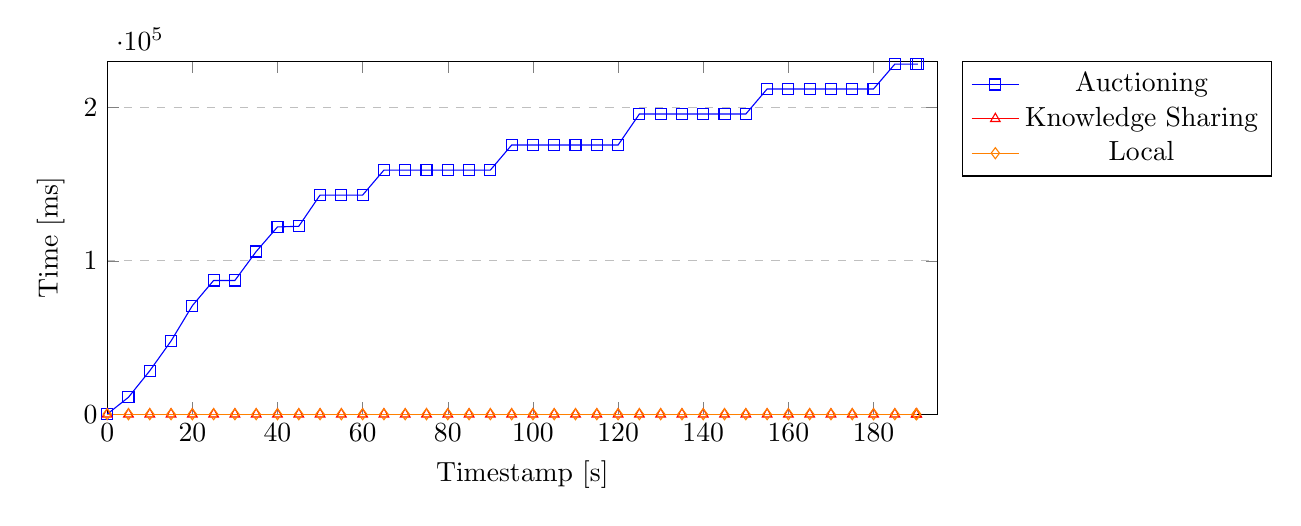
\begin{tikzpicture}
\begin{axis}[
    xlabel={Timestamp [s]},
    ylabel={Time [ms]},
    xmin=0, xmax=195000,
    ymin=0, ymax=230023,
    legend pos=outer north east,
    ymajorgrids=true,
    grid style=dashed,
    width=\textwidth,
    height=0.5\textwidth,
    scaled x ticks=base 10:-3,
    xtick scale label code/.code={}
]

	\addplot[color=blue,mark=square] coordinates {
        (0,0)(5000,11025)(10000,28282)(15000,47709)(20000,70713)(25000,87182)(30000,87182)(35000,106048)(40000,122066)(45000,122489)(50000,142841)(55000,142841)(60000,142841)(65000,159124)(70000,159124)(75000,159124)(80000,159124)(85000,159124)(90000,159124)(95000,175471)(100000,175471)(105000,175471)(110000,175471)(115000,175471)(120000,175471)(125000,195658)(130000,195658)(135000,195658)(140000,195658)(145000,195658)(150000,195658)(155000,212013)(160000,212013)(165000,212013)(170000,212013)(175000,212013)(180000,212013)(185000,228231)(190000,228231)(190439,228231)
    };
    \addlegendentry{Auctioning}
	\addplot[color=red,mark=triangle] coordinates {
        (0,0)(5000,0)(10000,0)(15000,0)(20000,0)(25000,0)(30000,0)(35000,0)(40000,0)(45000,0)(50000,0)(55000,0)(60000,0)(65000,0)(70000,0)(75000,0)(80000,0)(85000,0)(90000,0)(95000,0)(100000,0)(105000,0)(110000,0)(115000,0)(120000,0)(125000,0)(130000,0)(135000,0)(140000,0)(145000,0)(150000,0)(155000,0)(160000,0)(165000,0)(170000,0)(175000,0)(180000,0)(185000,0)(190000,0)(190147,0)
    };
    \addlegendentry{Knowledge Sharing}
	\addplot[color=orange,mark=diamond] coordinates {
        (0,0)(5000,0)(10000,0)(15000,0)(20000,0)(25000,0)(30000,0)(35000,0)(40000,0)(45000,0)(50000,0)(55000,0)(60000,0)(65000,0)(70000,0)(75000,0)(80000,0)(85000,0)(90000,0)(95000,0)(100000,0)(105000,0)(110000,0)(115000,0)(120000,0)(125000,0)(130000,0)(135000,0)(140000,0)(145000,0)(150000,0)(155000,0)(160000,0)(165000,0)(170000,0)(175000,0)(180000,0)(185000,0)(190000,0)(190136,0)
    };
    \addlegendentry{Local}




\end{axis}
\end{tikzpicture}
    \caption{Graph showing the sum of time spent auctioning by agents in the scenario where no changes are made overtime.}
    \label{fig:auctioning-time-no-change}
\end{figure}

Figure \ref{fig:auctioning-time-no-change} shows that the auctioning agents is the only agent that spends time auctioning. This is to be expected, as the auctioning agents are the only agents that can auction.

\begin{figure}[H]
    \centering
        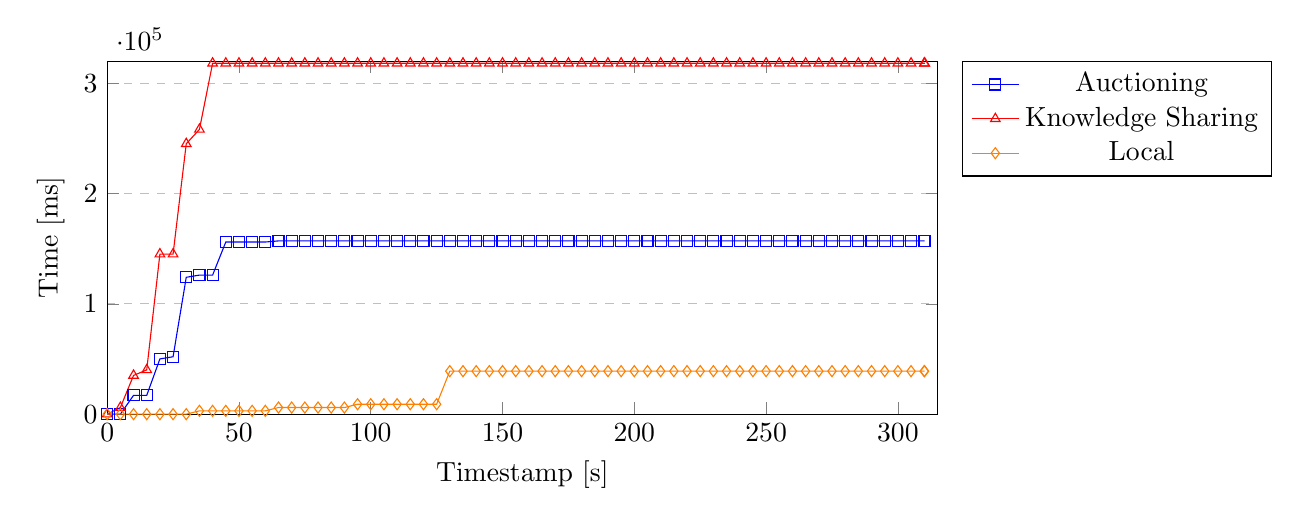
\begin{tikzpicture}
\begin{axis}[
    xlabel={Timestamp [s]},
    ylabel={Time [ms]},
    xmin=0, xmax=315000,
    ymin=0, ymax=320032,
    legend pos=outer north east,
    ymajorgrids=true,
    grid style=dashed,
    width=\textwidth,
    height=0.5\textwidth,
    scaled x ticks=base 10:-3,
    xtick scale label code/.code={}
]

	\addplot[color=blue,mark=square] coordinates {
        (0,0)(5000,0)(10000,17072)(15000,17072)(20000,50094)(25000,52106)(30000,124138)(35000,126144)(40000,126144)(45000,156154)(50000,156154)(55000,156154)(60000,156154)(65000,157158)(70000,157158)(75000,157158)(80000,157158)(85000,157158)(90000,157158)(95000,157158)(100000,157158)(105000,157158)(110000,157158)(115000,157158)(120000,157158)(125000,157158)(130000,157158)(135000,157158)(140000,157158)(145000,157158)(150000,157158)(155000,157158)(160000,157158)(165000,157158)(170000,157158)(175000,157158)(180000,157158)(185000,157158)(190000,157158)(195000,157158)(200000,157158)(205000,157158)(210000,157158)(215000,157158)(220000,157158)(225000,157158)(230000,157158)(235000,157158)(240000,157158)(245000,157158)(250000,157158)(255000,157158)(260000,157158)(265000,157158)(270000,157158)(275000,157158)(280000,157158)(285000,157158)(290000,157158)(295000,157158)(300000,157158)(305000,157158)(310000,157158)(310159,157158)
    };
    \addlegendentry{Auctioning}
	\addplot[color=red,mark=triangle] coordinates {
        (0,0)(5000,6039)(10000,35135)(15000,40149)(20000,145217)(25000,145217)(30000,245261)(35000,258272)(40000,318293)(45000,318293)(50000,318293)(55000,318293)(60000,318293)(65000,318293)(70000,318293)(75000,318293)(80000,318293)(85000,318293)(90000,318293)(95000,318293)(100000,318293)(105000,318293)(110000,318293)(115000,318293)(120000,318293)(125000,318293)(130000,318293)(135000,318293)(140000,318293)(145000,318293)(150000,318293)(155000,318293)(160000,318293)(165000,318293)(170000,318293)(175000,318293)(180000,318293)(185000,318293)(190000,318293)(195000,318293)(200000,318293)(205000,318293)(210000,318293)(215000,318293)(220000,318293)(225000,318293)(230000,318293)(235000,318293)(240000,318293)(245000,318293)(250000,318293)(255000,318293)(260000,318293)(265000,318293)(270000,318293)(275000,318293)(280000,318293)(285000,318293)(290000,318293)(295000,318293)(300000,318293)(305000,318293)(310000,318293)(310212,318293)
    };
    \addlegendentry{Knowledge Sharing}
	\addplot[color=orange,mark=diamond] coordinates {
        (0,0)(5000,0)(10000,0)(15000,0)(20000,0)(25000,0)(30000,0)(35000,3012)(40000,3012)(45000,3012)(50000,3012)(55000,3012)(60000,3012)(65000,6020)(70000,6020)(75000,6020)(80000,6020)(85000,6020)(90000,6020)(95000,9026)(100000,9026)(105000,9026)(110000,9026)(115000,9026)(120000,9026)(125000,9026)(130000,39035)(135000,39035)(140000,39035)(145000,39035)(150000,39035)(155000,39035)(160000,39035)(165000,39035)(170000,39035)(175000,39035)(180000,39035)(185000,39035)(190000,39035)(195000,39035)(200000,39035)(205000,39035)(210000,39035)(215000,39035)(220000,39035)(225000,39035)(230000,39035)(235000,39035)(240000,39035)(245000,39035)(250000,39035)(255000,39035)(260000,39035)(265000,39035)(270000,39035)(275000,39035)(280000,39035)(285000,39035)(290000,39035)(295000,39035)(300000,39035)(305000,39035)(310000,39035)(310137,39035)
    };
    \addlegendentry{Local}




\end{axis}
\end{tikzpicture}
    \caption{Graph showing the sum of time spent adapting by agents in the scenario where no changes are made overtime.}
    \label{fig:adapting-time-no-change}
\end{figure}

Figure \ref{fig:adapting-time-no-change} shows that the auctioning and knowledge-sharing agents spend roughly the same amount of time adapting in the early phases of the scenario. This is inline with the amount of adaptations applied. After roughly $100$ seconds, the knowledge-sharing agent applies one last adaptation to update the OS-version, which takes $10$ seconds in our simulation time. After this, the knowledge-sharing agent does not apply any more adaptations.
